\subsection{UCW6 - Proposta profilo TikTok}
\begin{figure}[!h]
\centering
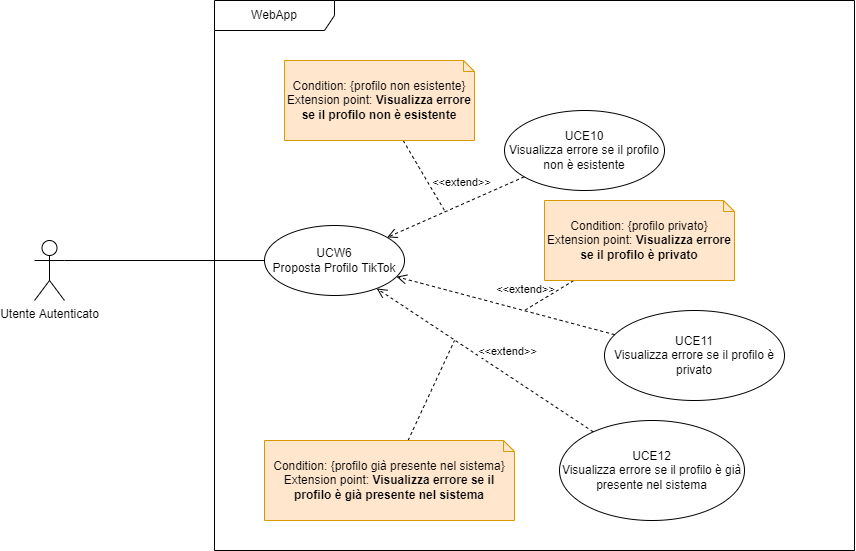
\includegraphics[scale=0.5]{UC_images/UCW6.png}
\caption{UCW6 - Proposta profilo TikTok}
\end{figure}
\begin{itemize}
	\item \textbf{Descrizione}: L'utente autenticato propone uno specifico profilo TikTok da cui effettuare il crawling dei dati.
    \item \textbf{Attore primario}: Utente autenticato.
    \item \textbf{Precondizione}: Il sistema possiede una lista di profili TikTok da cui effettuare il crawling dei dati.
    \item \textbf{Postcondizione}: Alla lista di profili da cui effettuare il crawling viene aggiunto il profilo indicato dall’utente e tutti i profili pubblici seguiti dal profilo suggerito.
    \item \textbf{Scenario principale}: 
    \begin{enumerate}
        \item L'utente autenticato accede al sistema;
        \item L’utente seleziona la funzionalità suggerisci un profilo TikTok;
        \item L’utente inserisce uno username valido di un profilo TikTok pubblico.
    \end{enumerate}
    \item \textbf{Estensioni}:
    \begin{itemize}
        \item Nel caso in cui l’utente inserisce uno username non esistente:
        \begin{enumerate}
            \item Lo username non viene inserito nella lista;
            \item Viene visualizzato un messaggio di errore nella proposta di profilo (UCE10 §);
            \item Viene fornita all’utente la possibilità di modificare lo username inserito.
        \end{enumerate}
        \item Nel caso in cui l’utente inserisce lo username di un profilo privato:
        \begin{enumerate}
            \item Lo username non viene inserito nella lista;
            \item Viene visualizzato un messaggio di errore nella proposta di profilo (UCE11 §).
        \end{enumerate}
        \item Nel caso in cui viene inserito lo username di un profilo pubblico già presente nel sistema:
        \begin{enumerate}
            \item Lo username non viene inserito nella lista.
            \item Viene visualizzato un messaggio di errore nella proposta di profilo (UCE12 §).
        \end{enumerate} 
    \end{itemize}
\end{itemize}

\pagebreak